\chapter{Request Replay Communication}
When we are dealing with client-server architecture, the form of \textbf{request-reply} communication is supported. In this type of communication, client and server exchange messages, described as \textit{send} and \textit{receive} operations, which can be \underline{datagrams} if using \textbf{UDP}, \underline{streams} for \textbf{TCP}.

\begin{figure}[!h]
    \centering
    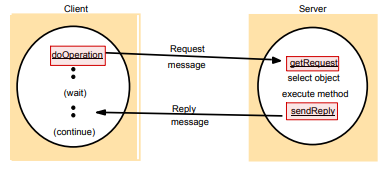
\includegraphics[width=.7\linewidth]{images/requestReplayCommunication/requestreplaycomm.png}
    \caption{Request Reply Communication}
\end{figure}

\section{Primitives}
The request/reply protocol is composed of \textbf{three primitives}, the way in which these 3 functions are \textbf{implemented} correspond to the \textbf{choice} of a space semantic provided by the communication system.
\begin{itemize}
    \item \textbf{doOperation:} used by the \textbf{client} to invoke remote operations and receiving the reply, specifying:
        \begin{itemize}
            \item The remote server
            \item The operation to be invoked
            \item The arguments of that operation 
        \end{itemize}
    The \textbf{client} is usually \textbf{blocked} until the server performs the requested operation since this type of communication is \textbf{synchronous} in the normal case. Asynchronous request-reply communication is rare, but it can exists, and it might be useful in situations where clients are allowed to retrieve replies later
    \item \textbf{getRequest:} used by the server process to receive requests
    \item \textbf{sendReply:} method used by the \textbf{server} to reply to the client when it has finished to invoke the requested operation. Then the \textbf{client} which receives the reply from the server is unblocked
\end{itemize}
The information transmitted in a request or reply  message is shown below:

\begin{figure}[!h]
    \centering
    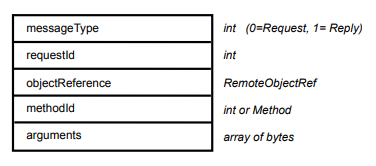
\includegraphics[width=.7\linewidth]{images/requestReplayCommunication/informatioTransmitted.png}
    \caption{Transmitted Infrmation}
\end{figure}

\begin{itemize}
    \item \textbf{messageType:} indicates the type of the message, if it is a \textit{request} or a \textit{reply} message
    \item \textbf{requestID:} is the message identifier. doOperation generates  requestId for each message and the server remembers these identifiers
    \item \textbf{objectReference:} is a remote object
    \item \textbf{methodId:} is an identifier for the operation to be invoked
\end{itemize}
Notice that in \textbf{request-reply} communication each message has a \textbf{unique message identifie}r by which it may be referenced. This message identifier is composed by:
\begin{itemize}
    \item A \underline{requestId} which is a sequence of integers
    \item And an \underline{identifier} for the sender process, to be unique in the distributed system
\end{itemize}

\section{Reliability and Faults in Request-Reply}
Now we face the faults in the request-reply communication, in particular if the \textbf{primitives} are implemented over \textbf{UDP protocol}, they suffer from:
\begin{itemize}
    \item Order of delivering not guaranteed
    \item Loss of message
    \item Process failures
\end{itemize}
In order to cope with these problems, \textit{doOperation} can use a \textbf{timeout:}
\begin{itemize}
    \item When the \textit{client} is \textbf{waiting} for the \textit{server’s reply}
    \item After a timeout, \textit{doOperation} sends the request message repeatedly until either it gets a reply or it is sure that the delay is due to lack of response from the server rather than to lost messages.
    The server has to have a \textbf{duplicate filtering strategy} thus when the server receives several request messages as it happens using the timeout, it should recognize multiple messages with the same request identifier and filter out the duplicates
\end{itemize}
Another problem can be the \textbf{re-execution} of the operations:
\begin{itemize}
    \item If the \textbf{reply from the server} has been \textbf{lost}, the server should execute the operation again to obtain the result unless it has stored the interested result
    \item The \textbf{history of transmitted reply messages} can be maintained by a table, but this could fill the memory
        \begin{itemize}
            \item The \textit{client} can make only \textbf{one request at a time}, so the server can interpret each request as acknowledgement of its previous reply, so the history needs to contain only the last reply message sent to each client
            \item However periodically the \textbf{messages in the history are discarded} after a period of time, because the client process can terminate and does not send the acknowledgement
        \end{itemize}
\end{itemize}

\section{Remote Procedure Call}
In RPC, procedures on remote machines can be called as if they are procedures in the local address space. In particular \textit{Interface definition languages (IDLs)} are designed to allow procedures implemented in different languages to invoke one another. The following point list describe the the remote invocation mechanism:
\begin{enumerate}
    \item The \textbf{Client calls the STUB} in normal state
    \item Client STUB \textbf{builds} the \textbf{request} message, parameter marshalling, calling the OS to make the call
    \item \textbf{OS sends} the message to the server
    \item \textbf{Server} node \textbf{receives} it, and passes to the Server STUB
    \item \textbf{Server STUB unmarshalling} of the parameters, \textbf{building the reply} message and passing th the OS for the reply
    \item The message is \textbf{sent} to the client
    \item The \textbf{Client STUB} receives the message
    \item Client STUB \textbf{unmarshalling, result passing} to the client
\end{enumerate}

\begin{figure}[!htb]
    \begin{minipage}{0.48\textwidth}
        \centering
        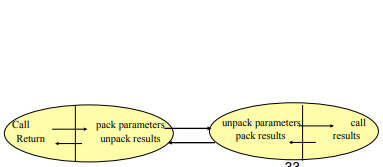
\includegraphics[width=.9\linewidth]{images/requestReplayCommunication/rpc1.png}
    \end{minipage}\hfill
    \begin{minipage}{0.48\textwidth} 
        \centering
        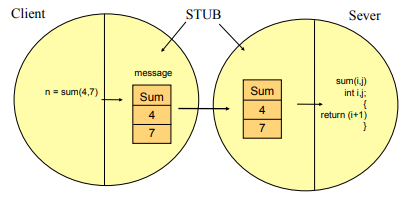
\includegraphics[width=.9\linewidth]{images/requestReplayCommunication/rpc2.png}
    \end{minipage}
\end{figure}
The primitives of request-reply protocols can be \textbf{implemented in different ways} to provide different delivery guarantees:
\begin{itemize}
    \item \textbf{Retry request message:} asking to retransmit the request message until either a reply is received or the server reasonably considered failed
    \item \textbf{Duplicate filtering:} filtering out duplicate requests at the server
    \item \textbf{Retransmission of results:} keeping a \textbf{history of result messages} to enable lost results to be retransmitted without re-executing the operations at the server
\end{itemize}

\subsection{RPC design issues}
The RPC has three main design issues:
\begin{itemize}
    \item \textbf{Parameter passing:}
        \begin{itemize}
            \item \textit{Call by value:} the parameter value is copied in the file, and if this is modified, this has no effect on the original variable
            \item \textit{Call by reference:} the reference to the variable is copied, the called procedure HAS access to the variable and the modifications directly affect the calling program
            \item \textit{Call by value-result:} the value of the variable is copied n the file as in the call by value, then it is copied back to it after the call, rewriting the original result
        \end{itemize}
    \item \textbf{Binding:}
        \begin{enumerate}
            \item \textit{Static:} write the client program for a specific server on a specific machine
            \item \textit{Dynamic:} locate the server at \textbf{run time}
        \end{enumerate}
    \item \textbf{Fault managements:}
        \begin{itemize}
            \item \textit{Communication:} the working processes can be not able to temporary communicate
            \item \textit{Node crash:} possible recover
        \end{itemize}
\end{itemize}
 
\subsection{Semantic in RPC}
Before introducing the semantic we have to clarify that:
\begin{itemize}
    \item \textbf{Normal Termination (NT):} when the client receives the message from the server
    \item \textbf{Abnormal termination (AT):} when the client \textbf{DOES NOT receive the reply}, so either it has not received any message or has received an unknown address (AU)
\end{itemize}
Semantics:
\begin{itemize}
    \item \textbf{Maybe / exactly one:} RPC may be executed \textbf{once or not at all}. If the result message has not been received after a timeout and there are no retries, it is uncertain whether the procedure has been executed
        \begin{itemize}
            \item NT: the call has been executed once
            \item AT: the call has \textbf{NOT} been executed once
        \end{itemize}
    Difficult to implement
    \item \textbf{At least once:} it is achieved by the \textbf{retransmission of request messages} as idempotent operation. The client calls with timeout, and if the answer has not arrived yet, it tries again repeating the attempts a finite number of times
        \begin{itemize}
            \item NT: the call has been executed once or more than once
            \item AT: the call has \textbf{NOT} been executed once
        \end{itemize}
    \item \textbf{At most once semantics:} it is achieved by retries masking any omission failures of the requests
        \begin{itemize}
            \item NT: the call has been executed once
            \item AT: the call has \textbf{NOT} been executed once or it has been \textbf{partially} executed or it has been executed \textbf{more than once}
        \end{itemize}
    Relatively easy to implement
\end{itemize}

\subsection{RPC fault management and semantics}
The faults can be classified into two main categories:
\begin{itemize}
    \item \textbf{Communication:} working processes can not be able to communicate temporarily
    \item \textbf{Node crash:} possible recovers, we should build the correct semantics
\end{itemize}
In particular, the possible faults are the following:
\begin{itemize}
    \item The cannot locate the server process
    \item Loss of the client request message
    \item Loss of the reply of the server
    \item Server crash during the call
    \item Client crash during the call
\end{itemize}
We can try to distinguish \textbf{several situation} in which the client \textit{sends} the request and then the \textbf{timeout reaches the deadline while it waits for the answer:}
\begin{itemize}
    \item If the \textbf{client does not try again:} semantics RPC is \underline{maybe}
    \item If the \textbf{client tries until it gets a reply} and the \textbf{answer is AU}, the call has \textit{abnormal termination} with RPC semantics \underline{exactly once}
    \item If the \textbf{client tries until it gets a reply} and the \textbf{answer is the reply}, if the server has \textbf{no memory of previous execution}, the server can \textbf{execute the duplicated requests} and so RPC semantics is at \underline{least once}
    \item If the \textbf{server keeps the result of the last execution in a buffer}, in case of \textbf{duplicated} requests it is \textbf{detected} and it \textbf{sends again the result}; RPC semantics is at \underline{most once}
\end{itemize}

Furthermore we should distinguish the two types of crashes: 
\begin{itemize}
    \item \textit{During} the execution
    \item \textit{Before} the execution
    \item \textit{After} the execution
\end{itemize}

\begin{figure}[!h]
    \centering
    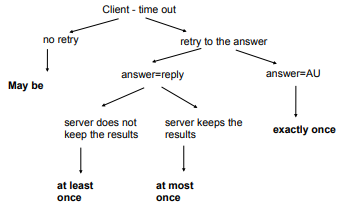
\includegraphics[width=.7\linewidth]{images/requestReplayCommunication/faultmanagement.png}
    \caption{Fault Management and Semantics}
\end{figure}

\subsection{RPC semantic and server crash}
Crashing of servers can happen during or after the execution phase, and this is totally \textbf{transparent to the client}. The unique information that it has is the fact that the timeout occurs. \textbf{Semantics exactly once} is very difficult to reach on a distributed system, it has to satisfy the behaviour \textbf{"all or nothing"}:
\begin{enumerate}
    \item Meaning that in case of normal \textbf{termination} the request is \textbf{executed only once}, otherwise in case of \textbf{abnormal termination no execution} of the request
\end{enumerate}
In the presence of server crash provided exactly once semantic it is necessary to use \textbf{atomic actions}, which allow client and server to coordinate their action in order to guarantee \textbf{"all or nothing"} property. But this approach is not practicable, and what is essentially done is to implement at \underline{most once semantics}.
Summary of the two semantics:
\begin{itemize}
    \item \textbf{At least one RPC:}
        \begin{itemize}
            \item \textit{Client:}
                \begin{itemize}
                    \item Send request setting a timeout
                    \item If the timeout is over try again until it receives an answer or for a finite number of times
                \end{itemize}
            \item \textit{Server:}
                \begin{itemize}
                    \item Executes the received call and sends the answer
                    \item It does not keep memory of the previous calls
                \end{itemize}
        \end{itemize}
    \item \textbf{At most one RPC:}
        \begin{itemize}
            \item \textit{Client:}
                \begin{itemize}
                    \item Send request setting a timeout
                    \item If the timeout is over try again until it receives an answer or for a finite number of times
                \end{itemize}
            \item \textit{Server:}
                \begin{itemize}
                    \item It store an history of the last call for each client
                    \item For each request it checks whether it is a new one and only in this case executes it. Otherwise it sends the previous computed result. Only in case of a crash of the server this state is lost
                \end{itemize}
        \end{itemize}
\end{itemize}

\subsection{RPC and client crash}
\begin{itemize}
    \item If a client is subject to a crash after sending a request that has been executed by the server, the execution is \textbf{called orphans}
    \item They consume resources (execution, memory, etc)
    \item The orphans create consistency problems and they interfere with the normal execution
\end{itemize}

\begin{figure}[!h]
    \centering
    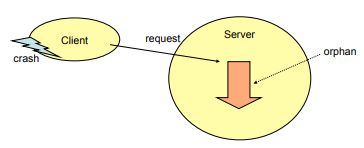
\includegraphics[width=.7\linewidth]{images/requestReplayCommunication/orphan.png}
    \caption{Client Crash}
\end{figure}
\newpage

We can manage the \textbf{orphans} in two way:
\begin{itemize}
    \item \textbf{Duplicate check:}
        \begin{itemize}
            \item The \textbf{server} as soon as receives a new request \textbf{checks} whether it is already in execution from the same node a previous request from the same client
            \item If so it should \textbf{terminate} or abort the \textbf{previous call} before executing the current one
        \end{itemize}
    \item \textbf{Check of client vitality:}
        \begin{itemize}
            \item A \textbf{server} should \textbf{periodically checks} whether the \textbf{clients} are \textit{“alive”}
            \item If one suspects a fault of the client, then one should \textbf{terminate} or abort the orphans
        \end{itemize}
\end{itemize}